% Source: tex/chapters/ch05/06_テスト技法.tex
\subsubsection{欠陥ベース技法とミューテーション技法}
欠陥ベーステストは、あり得る欠陥の種類を想定し、それを露出させるテストケースを作る。欠陥分類や直交欠陥分類を使うと、欠陥の意味情報を整理し、根本原因分析を短縮できる。

ミューテーションテストは、SUT をわずかに変更した変異体を多数作り、テストスイートがそれらの違いを検出できるかを評価する技法である。テストが変異体を見破れば、その変異体は殺されたという。変異体を多く殺せるテストスイートほど、欠陥検出能力が高いと考える。近年は、機械学習システムのテストで、入力を変化させて出力関係を見るメタモルフィックテストにも関連する。

\begin{figure}[htbp]
\centering
\IfFileExists{assets/generated_figures/ch05/fig-ch05-10.png}{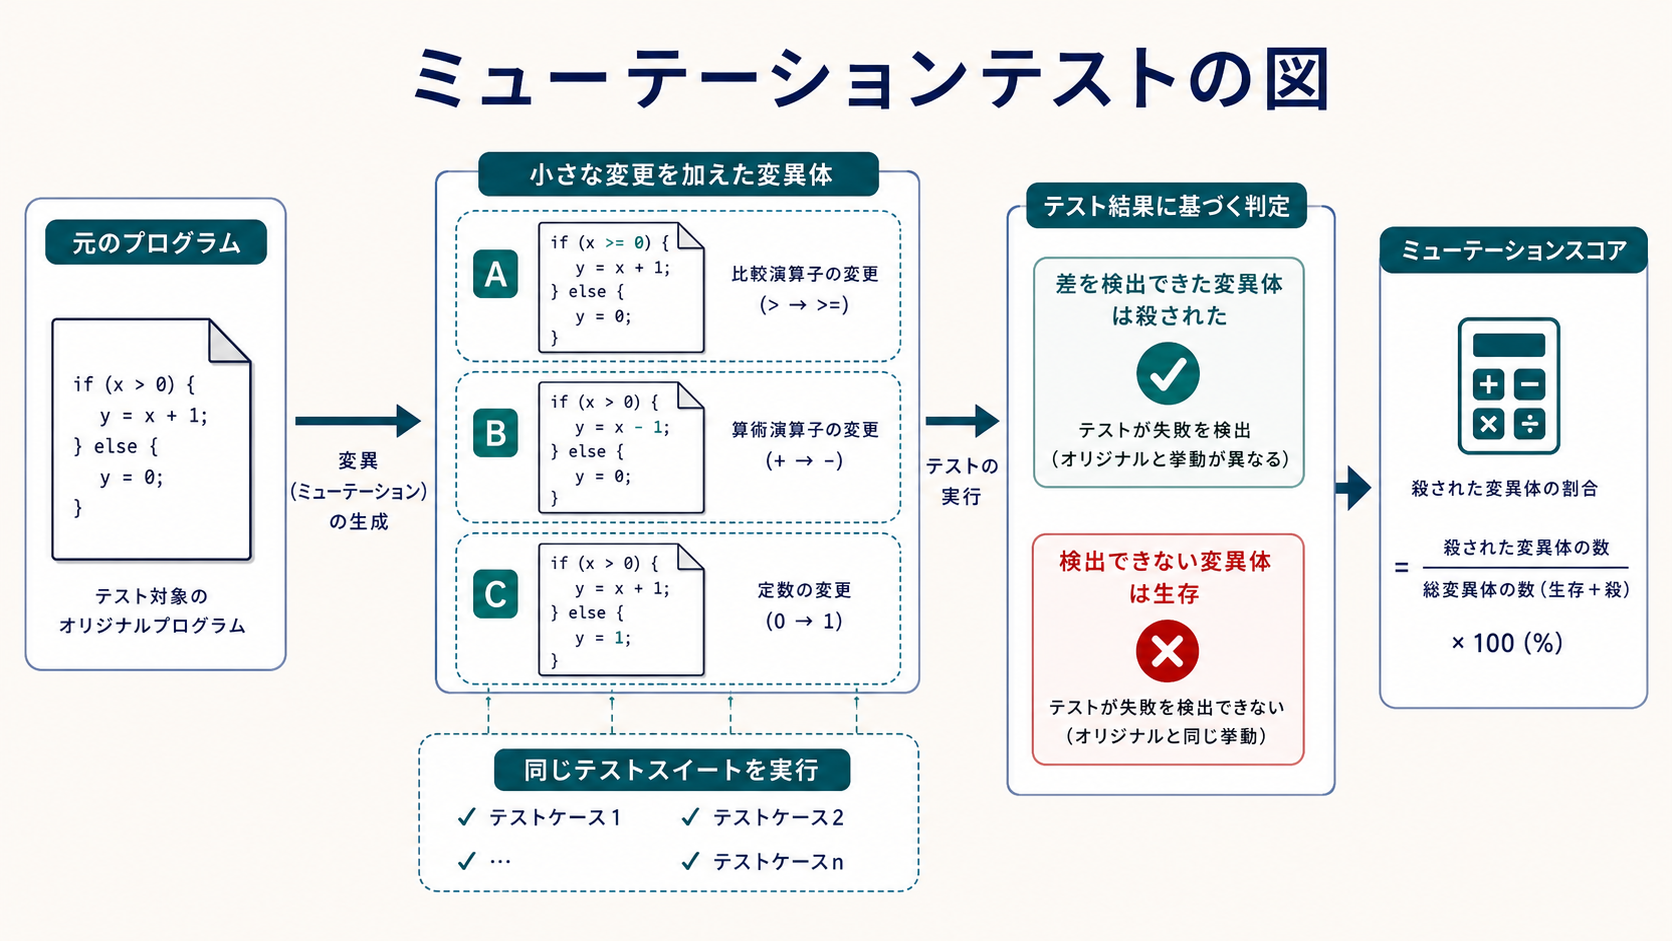
\includegraphics[width=0.96\linewidth]{assets/generated_figures/ch05/fig-ch05-10.png}}{\fbox{\parbox[c][48mm][c]{0.9\linewidth}{\centering 画像生成待ち\\ミューテーションテストの図}}}
\caption{ミューテーションテストの図}
\label{fig:ch05-10}
\end{figure}
